	\documentclass{beamer}[aspectratio=169]
	\usepackage[utf8]{inputenc}
	\usepackage[russian]{babel}
    %\usepackage{graphicx} 
    \usepackage{booktabs} 
    \usepackage{beamerthemesplit}
    \setbeamertemplate{footline}[frame number]
    \usepackage{color} %% это для отображения цвета в коде
	\usepackage{listings} 
	\usepackage{multimedia}
\usepackage{media9}	
	
	
	%\usepackage[dvips]{graphicx}
	%\usepackage{graphicx}
	%\DeclareGraphicsExtensions{.png,.jpg,.svg}%какое расширение будем использовать 
	\usepackage{pdflscape,multicol,blindtext}
	\usepackage{amsmath}
	\usepackage{subcaption}
	\usepackage{pgfplots}
	\usepackage{hyperref}
	\usepackage{tikz}
	\usepackage{adjustbox}
	\usepackage{listings}
	\usepackage{longtable}
	%\usepackage{fullpage}
	
	%\usetikzlibrary{}
    \usetheme{PaloAlto}
	\usecolortheme{rose}
	
	\makeatletter
\beamer@headheight=1.7\baselineskip     %controls the height of the headline, default is 2.5    
\makeatother
	
	
	
	
	\title[Презентация]{Инструменты для оформления научных статей и презентаций на примере \LaTeX'}
	\institute{КемГУ}
	\author{Дмитрий Басалаев \and Буданцев Артём \and Болковая Полина}
	\date{28.05.2021}
	
\begin{document}
\newlength\someheight
\setlength\someheight{2cm}



\begin{frame}
\maketitle
\end{frame}


\section{Общие цели и задачи}
\begin{frame}{Общие цели и задачи}
\transdissolve
\textbf{Цель:} Составить презентацию и отчет о проделанной работе при помощи LateX. Ознакомить студентов с его базовыми возможностями.

\begin{center}
\textbf{Наш репозиторий}
\url{https://github.com/Antur1um/Practice-LateX.git}

\end{center}
\end{frame}

\section{План график}
\begin{frame}{План график}
\transboxout
\begin{tabular}{| l| p{6.7cm}|}
\hline {\bfseries \large Даты} & {\bfseries \large Действия}\\ \hline
03.02.21-11.03.21. & Изучение базы, установка необходимого софта,подготовка документации\\ \hline
12.03.21-26.03.21 & Изучение интерфейса в \TeX maker, набор простых текстов, спецсимволы \\ \hline
27.03.21-15.04.21 & Ввод математических формул, ввод матриц, спецсимволы  \\ \hline
16.04.21-28.04.21 & Работа с изображениями и встроенной графикой, построение графиков \\ \hline 
29.04.21-14.05.21 & Работа с ссылками,разметка страницы, различные окружения, работа с графикой и презентациями \\ \hline
15.05.21- & Разработка финального продукта, подготовка отчета. \\ \hline
\end{tabular}

\end{frame}
\section{Используемые программные средства}
\begin{frame}{Используемые программные средства}
\transwipe
\begin{figure}[h]
\begin{tabular}{cc}

\includegraphics[width=5cm,height=2cm]{texlive}
&

\includegraphics[width=4cm,height=4cm]{texmaker}
\end{tabular}
\end{figure}

\end{frame}

\begin{frame}
\section{Ход работы}
\subsection{Ввод формул}
\transwipe
Итак, мы приступили к вводу математических выражений и формул. Желая начать с чего-то простого, мы решили переписать школьную таблицу производных и интегралов.
\begin{figure}[h!]
\setlength{\fboxsep}{0pt}%
\setlength{\fboxrule}{1pt}%ширина рамки
\fbox{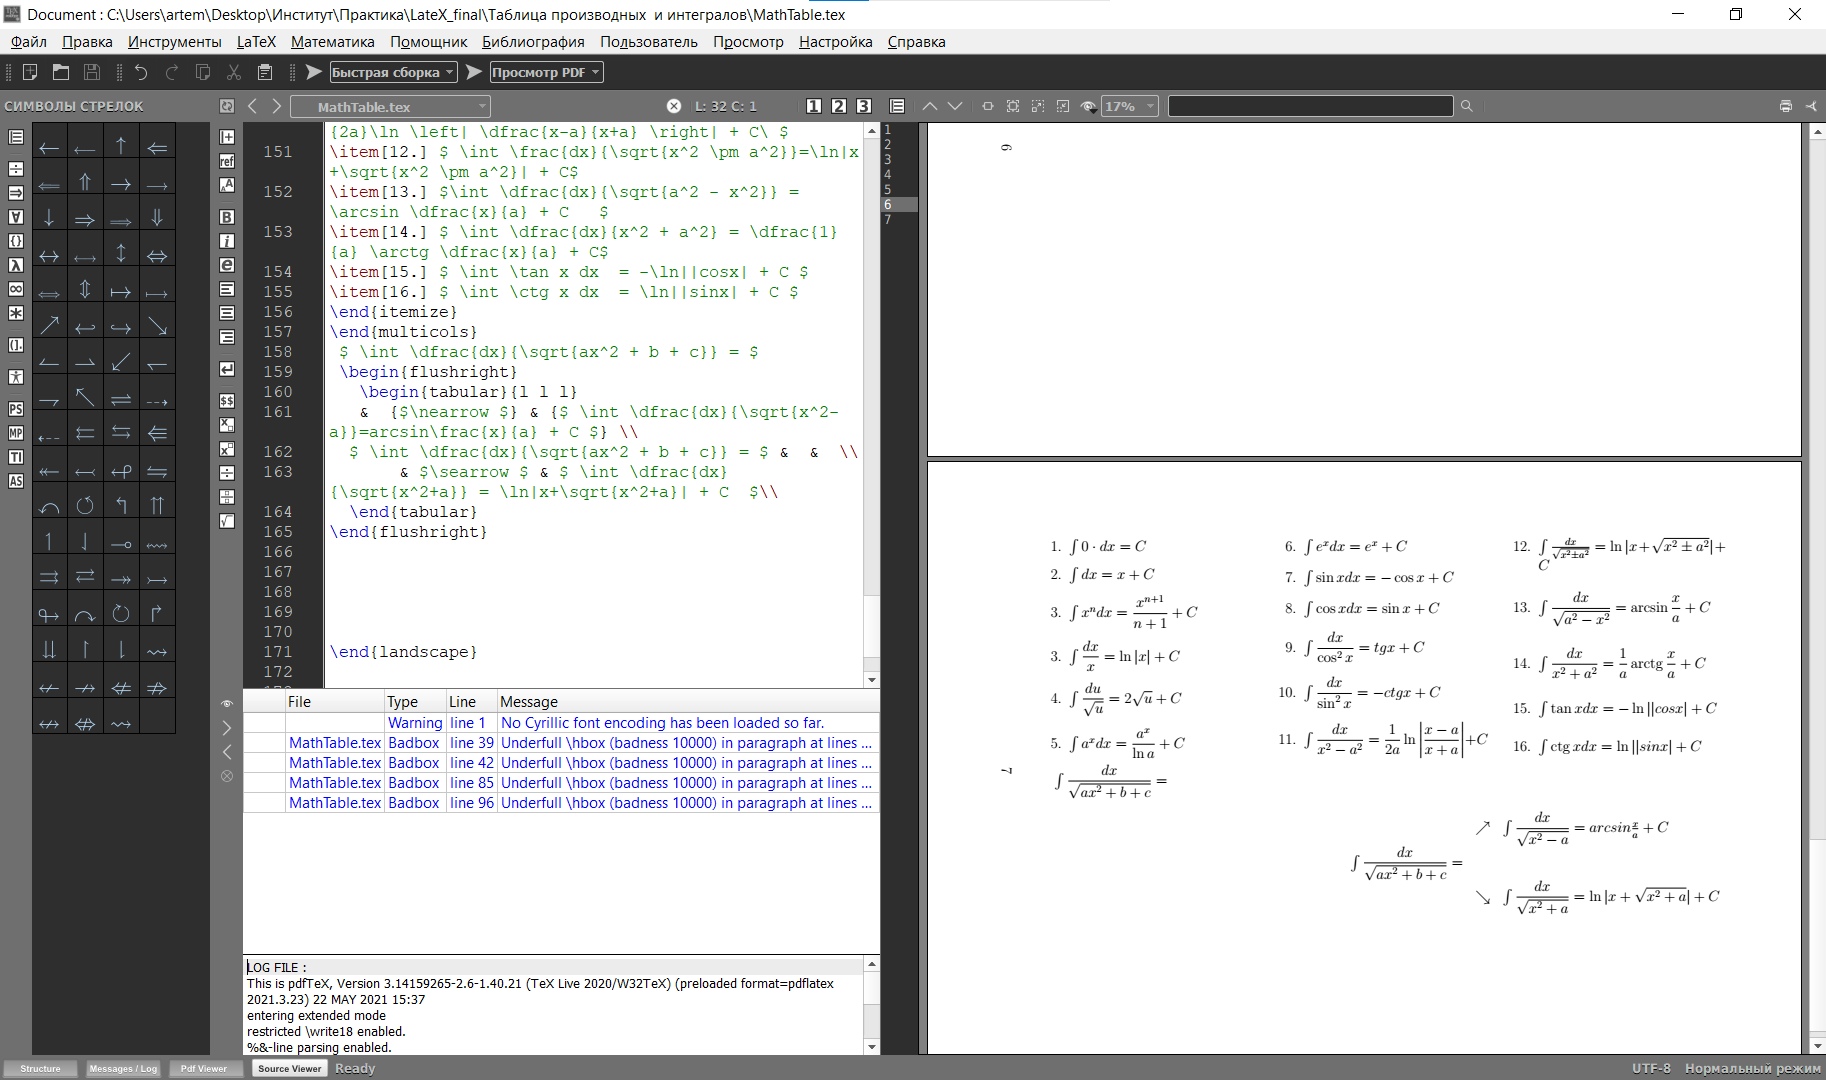
\includegraphics[width=10cm,height=6cm]{Example(1)}}%
\caption{Уже на этом этапе можно понять наскольно в \LaTeX \  проще и быстрее вводить математематические формулы}
\label{fig:image}
\end{figure}
\end{frame}


\begin{frame}
\transwipe
Итак, быстро убедившись, что ввод сложных математических формул не представляет трудностей, мы приступили к вводу матриц и других крупных объектов.
\begin{figure}[h!]
\setlength{\fboxsep}{0pt}%
\setlength{\fboxrule}{1pt}%ширина рамки
\fbox{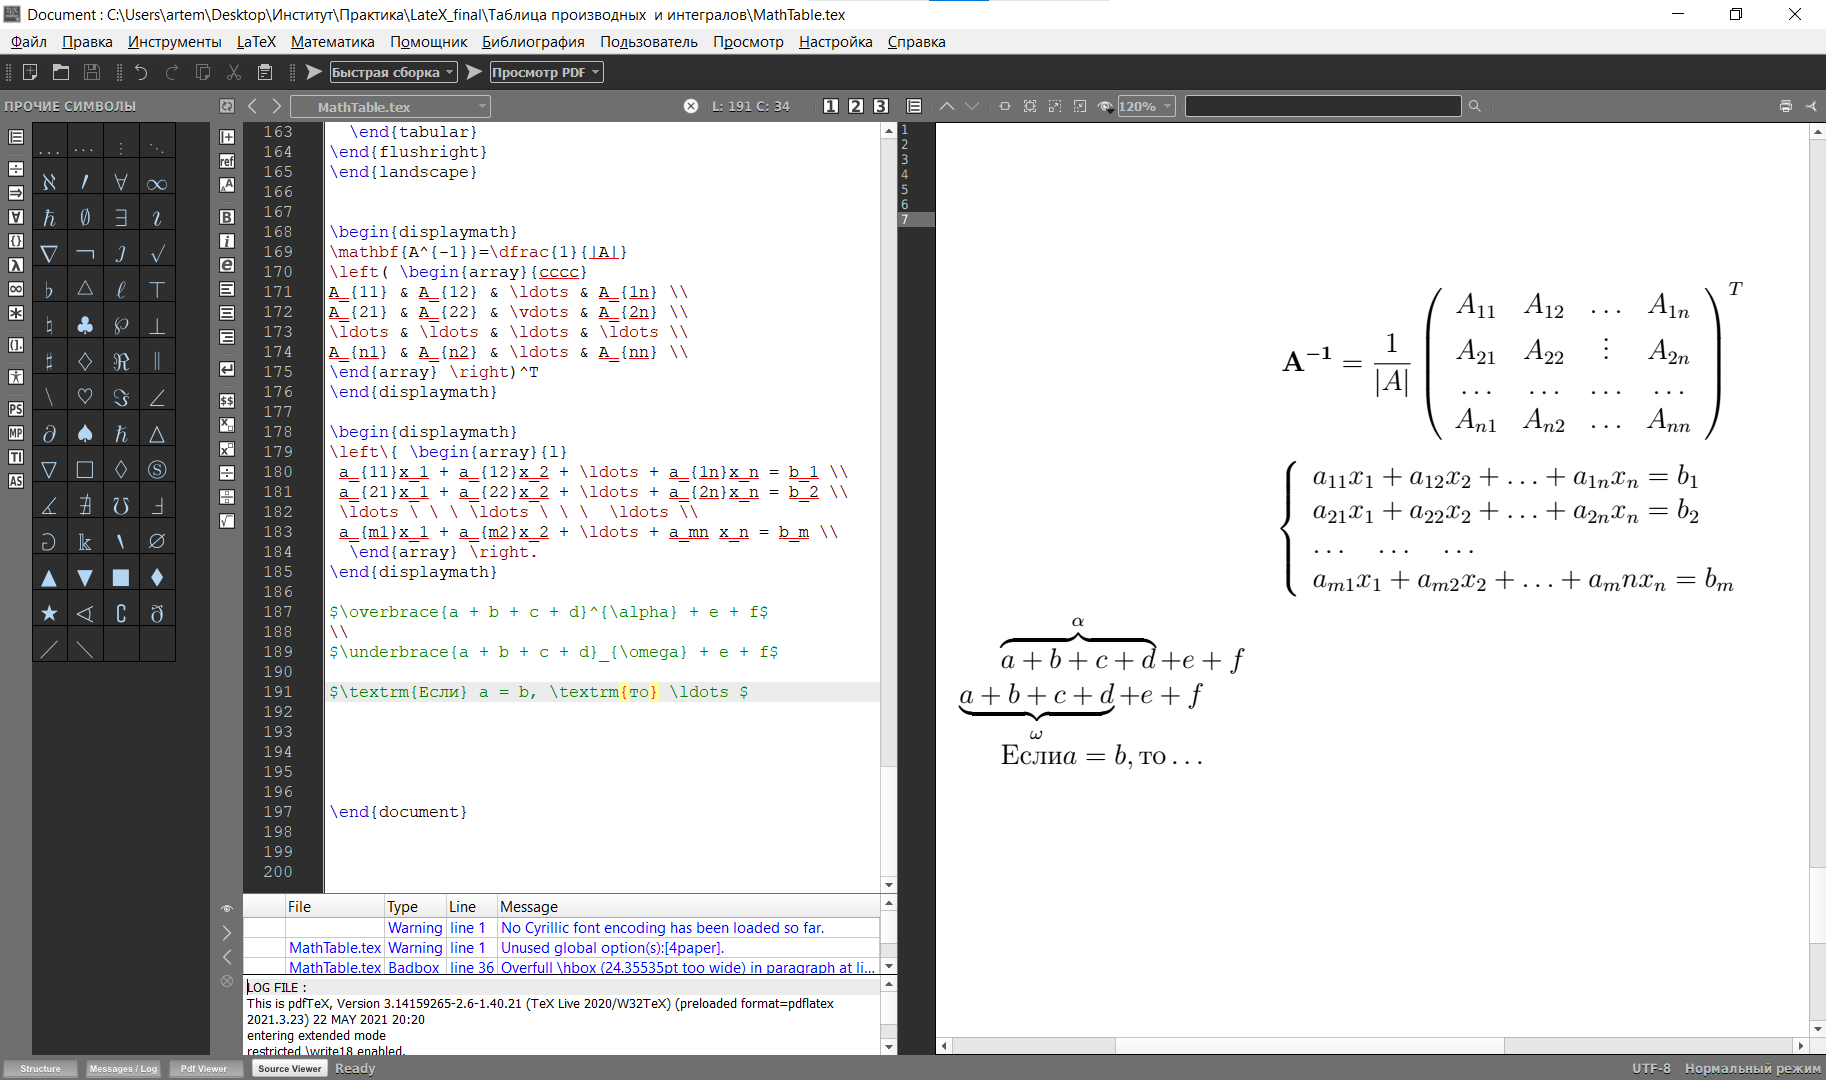
\includegraphics[width=6cm,height=3cm]{Matrrix(1)}}%
\caption{"Крупные" математические объекты}
\end{figure}
\end{frame}



\begin{frame}
\transwipe
Что же касается спец символов, в \LaTeX 'e их огромное количество, но раз уж речь идет о математике, то давайте попробуем собрать определение последовательности на языке " $\varepsilon \ \Delta $'
$$\lim_{x \rightarrow x_0}f(x) = A \  \Leftrightarrow \   \forall \ \varepsilon > 0,$$

$$\ \exists \delta \ >0, |\forall x \ 0<|x-x_0|<\delta \ \Rightarrow |f(x) - A|< \varepsilon   $$


$$\lim_{x \rightarrow 0}\frac{\sin x}{x} = 1  $$

$$\lim_{x \rightarrow \infty} \left( 1 + \frac{1}{x} \right)^x = e  $$

%$\lim_{x \rightarrow 0} \dfrac{sinx}{x} = 1$

\end{frame}




\begin{frame}[label=frame_A]{Простые формулы}
\transwipe
\begin{multicols}{3}
    \begin{itemize}
\item[1.] $ c' = 0 \  (c = const)  $
\item[2.] $ (x^n)' = nx^{n-1} $
\item[3.] $ (\sqrt{x})' = \dfrac{1}{2\sqrt{x}} $
\item[4.] $ (a^x)' = a^x\cdot  \ln{a} $
\item[5.] $ (e^x)' = e^x $
\item[6.] $ (\log_{a} x)' = \frac{1}{x\ln a} $
\item[7.] $ (\ln x)' = \frac{1}{x}  $ 
\item[8.] $(\sin \  x)' = \cos \ x  $ 
\item[9.] $(\cos \  x) = - \sin \ x  $ 
\item[10.] $ (\tan \ x)' = \dfrac{1}{\cos ^2 x}  $
\item[11.] $(\ctg)' = -\dfrac{1}{\sin^2 x}  $
\item[12.] $ (\arcsin \ x)' = \dfrac{1}{\sqrt{1 - x^2}}  $ 
\item[13.] $ (\arccos \ x)' = -\dfrac{1}{\sqrt{1 - x^2}}  $ 
\item[14.] $ (\arctan \ x)' = \dfrac{1}{1 + x^2} $
\item[15.] $ (arcctg  \ x)' = -\dfrac{1}{1 + x^2} $
\item[16.] $ (\sinh x)' = \cosh \ x $
\item[17.] $ (\cosh x)' = \sinh \ x $
\item[18.] $ (\tanh x)' = \dfrac{1}{\cosh^2 x}
 $
 \item[19.] $ (cth \  x)' = -\dfrac{1}{\sinh^2 x}
 $
\end{itemize}
\end{multicols}
\begin{center}
\hyperlink{list}{\beamerbutton Back}
\end{center}
\end{frame}

\begin{frame}[fragile]{Их исходный код}
\transwipe
\begin{adjustbox}{width=15cm,height=3.5cm,keepaspectratio}
 \begin{lstlisting}[language=Tex]

\item[1.] $ c' = 0 \  (c = const)  $
\item[2.] $ (x^n)' = nx^{n-1} $
\item[3.] $ (\sqrt{x})' = \dfrac{1}{2\sqrt{x}} $
\item[4.] $ (a^x)' = a^x\cdot  \ln{a} $
\item[5.] $ (e^x)' = e^x $
\item[6.] $ (\log_{a} x)' = \frac{1}{x\ln a} $
\item[7.] $ (\ln x)' = \frac{1}{x}  $ 
\item[8.] $(\sin \  x)' = \cos \ x  $ 
\item[9.] $(\cos \  x) = - \sin \ x  $ 
\item[10.] $ (\tan \ x)' = \dfrac{1}{\cos ^2 x}  $
\item[11.] $(\ctg)' = -\dfrac{1}{\sin^2 x}  $
\item[12.] $ (\arcsin \ x)' = \dfrac{1}{\sqrt{1 - x^2}}  $ 
\item[13.] $ (\arccos \ x)' = -\dfrac{1}{\sqrt{1 - x^2}}  $ 
\item[14.] $ (\arctan \ x)' = \dfrac{1}{1 + x^2} $
\item[15.] $ (arcctg  \ x)' = -\dfrac{1}{1 + x^2} $
\item[16.] $ (\sinh x)' = \cosh \ x $
\item[17.] $ (\cosh x)' = \sinh \ x $
\item[18.] $ (\tanh x)' = \dfrac{1}{\cosh^2 x}
 $
 \item[19.] $ (cth \  x)' = -\dfrac{1}{\sinh^2 x}
 $
\end{lstlisting}
\end{adjustbox}
\end{frame}

\begin{frame}[label=Frame]{Нестандартная формула}
\transwipe
\begin{tabular}{l l l} 
   &  {$\nearrow $} & {$ \int \dfrac{dx}{\sqrt{x^2-a}}=arcsin\frac{x}{a} + C $} \\
  $ \int \dfrac{dx}{\sqrt{ax^2 + b + c}} = $ &  &  \\ 
       & $\searrow $ & $ \int \dfrac{dx}{\sqrt{x^2+a}} = \ln|x+\sqrt{x^2+a}| + C  $\\ 
  \end{tabular}
\begin{center}
\hyperlink{Back}{\beamerbutton{Back}}
\end{center}
\end{frame}

\begin{frame}[fragile]{Исходный код}
\begin{adjustbox}{scale=0.5}
\begin{large}
\transwipe

 \begin{lstlisting}[language=Tex]
  \begin{tabular}{l l l} 
   &  {$\nearrow $} & {$ \int \dfrac{dx}{\sqrt{x^2-a}}=arcsin\frac{x}{a} + C $} \\
  $ \int \dfrac{dx}{\sqrt{ax^2 + b + c}} = $ &  &  \\ 
       & $\searrow $ & $ \int \dfrac{dx}{\sqrt{x^2+a}} = \ln|x+\sqrt{x^2+a}| + C  $\\ 
  \end{tabular}
\end{lstlisting}
\end{large}
\end{adjustbox}
 

\end{frame}

\begin{frame}{``Крупные' математические объекты}
\transwipe


\begin{displaymath}
\mathbf{A^{-1}}=\dfrac{1}{|A|}
\left( \begin{array}{cccc}
A_{11} & A_{12} & \ldots & A_{1n} \\
A_{21} & A_{22} & \vdots & A_{2n} \\
\ldots & \ldots & \ldots & \ldots \\
A_{n1} & A_{n2} & \ldots & A_{nn} \\
\end{array} \right)^T
\end{displaymath}
\vspace{1cm}
\begin{displaymath}
\left\{ \begin{array}{l}
 a_{11}x_1 + a_{12}x_2 + \ldots + a_{1n}x_n = b_1 \\
 a_{21}x_1 + a_{22}x_2 + \ldots + a_{2n}x_n = b_2 \\
 \ldots \ \ \ \ldots \ \ \  \ldots \\
 a_{m1}x_1 + a_{m2}x_2 + \ldots + a_mn x_n = b_m \\                    
  \end{array} \right.
\end{displaymath}

\end{frame}

\begin{frame}[fragile]{Исходный код}
\transwipe
\begin{adjustbox}{scale=0.7}
\begin{large}


 \begin{lstlisting}[language=Tex]
  \begin{displaymath}
\mathbf{A^{-1}}=\dfrac{1}{|A|}
\left( \begin{array}{cccc}
A_{11} & A_{12} & \ldots & A_{1n} \\
A_{21} & A_{22} & \vdots & A_{2n} \\
\ldots & \ldots & \ldots & \ldots \\
A_{n1} & A_{n2} & \ldots & A_{nn} \\
\end{array} \right)^T
\end{displaymath}
\vspace{1cm}
\begin{displaymath}
\left\{ \begin{array}{l}
 a_{11}x_1 + a_{12}x_2 + \ldots + a_{1n}x_n = b_1 \\
 a_{21}x_1 + a_{22}x_2 + \ldots + a_{2n}x_n = b_2 \\
 \ldots \ \ \ \ldots \ \ \  \ldots \\
 a_{m1}x_1 + a_{m2}x_2 + \ldots + a_mn x_n = b_m \\                    
  \end{array} \right.
\end{displaymath}

\end{lstlisting}
\end{large}
\end{adjustbox}


\end{frame}
\subsection{Работа с графикой и изображениями}
\begin{frame}{Использование пакета tikz}
\transwipe

\begin{tikzpicture}
\draw(0,0)--(1,0)--(1.5,-0.5)--(1.5,-2)--(1,-3.5)--(2.5,-4.5)--(3,-4.5)--(3,-4)--(2.5,-4)--(2,-3)--(3,-2.5)--(3.5,-3.5)--(4.5,-4)--(5,-4)--(5,-3.5)--(4.5,-3.5)--(4,-3)--(4,-2.5)--(4.5,-3)--(6.5,-3)--(7,-4.5)--(7.5,-5)--(8,-5)--(8,-4.5)--(7.5,-4.5)--(7.5,-3.5)--(8.5,-4.5)--(9,-4.5)--(9,-4)--(8.5,-4)--(8,-3)--(8.5,-3)--(9,-2.5)--(9,-1)--(8.5,-1.5)--(8,-1.5)--(7.5,-1)--(7.5,-2)--(7,-2)--(5,-1)--(4,-1)--(2.5,-1.5)--(2.5,-0.5)--(1.5,0.5)--(1,0.5)--cycle;
\end{tikzpicture}

\end{frame}

\begin{frame}{Исходный код}
\transwipe
$\backslash$ \textbf{begin\{tikzpicture\} }\\
$\backslash$\textbf{draw(0,0)--(1,0)--(1.5,-0.5)--(1.5,-2)--}\\
\textbf{(1,-3.5)--(2.5,-4.5)--(3,-4.5)}\\
\textbf{--(3,-4)--(2.5,-4)--(2,-3)}\\
\textbf{--(3,-2.5)--(3.5,-3.5)--(4.5,-4)}\\
\textbf{--(5,-4)--(5,-3.5)--(4.5,-3.5)}\\
\textbf{--(4,-3)--(4,-2.5)--(4.5,-3)}\\
\textbf{--(6.5,-3)--(7,-4.5)--(7.5,-5)--}\\
\textbf{(8,-5)--(8,-4.5)--(7.5,-4.5)}\\
\textbf{--(7.5,-3.5)--(8.5,-4.5)--(9,-4.5)}\\
\textbf{--(9,-4)--(8.5,-4)--(8,-3)--(8.5,-3)}\\
\textbf{--(9,-2.5)--(9,-1)--(8.5,-1.5)}\\
\textbf{--(8,-1.5)--(7.5,-1)--(7.5,-2)}\\
\textbf{--(7,-2)--(5,-1)--(4,-1)--(2.5,-1.5)}\\
\textbf{--(2.5,-0.5)--(1.5,0.5)--(1,0.5)--cycle;}\\
$\backslash$\textbf{ end \{ tikzpicture \}}\\
\end{frame}

\begin{frame}{Добавление подписей к прямым и углам}
\transwipe


\begin{tikzpicture}[scale=1.75]
\fill[left color=magenta, right color=yellow]
(0,0) -- node[below=3pt] {$a$} (4,0) --
node[right=5pt] {$b$} (4,3) --
cycle node[midway,above,sloped] {$c=\sqrt{a^2+b^2}$};
\node[below left] at (0,0) {\color{blue}$B$};
\node[below right] at (4,0) {\color{blue}$C$};
\node[above right] at (4,3) {\color{blue}$A$};
\end{tikzpicture}


\end{frame}

\begin{frame}[fragile]{Исходный код}
\begin{adjustbox}{scale=0.8}
\begin{large}
\transwipe

 \begin{lstlisting}[language=Tex]
  \begin{tikzpicture}[scale=1.75]
\fill[left color=magenta, right color=yellow]
(0,0) -- node[below=3pt] {$a$} (4,0) --
node[right=5pt] {$b$} (4,3) --
cycle node[midway,above,sloped] {$c=\sqrt{a^2+b^2}$};
\node[below left] at (0,0) {\color{blue}$B$};
\node[below right] at (4,0) {\color{blue}$C$};
\node[above right] at (4,3) {\color{blue}$A$};
\end{tikzpicture}

\end{lstlisting}
\end{large}
\end{adjustbox}
\end{frame}

\begin{frame}{Дуги окружности}


\begin{tabular}{ll}
$\backslash$ \textbf{begin\{tikzpicture\}} \\           
$\backslash$ \textbf{draw[Red,ultra thick](1,1) arc (20:60:2);}\\
$\backslash$ \textbf{draw[Red,ultra thick](0,0) arc (20:60:1.5);}\\
$\backslash$ \textbf{draw[thick](2,1) arc (0:-120:2);}\\
$\backslash$ \textbf{end\{tikzpicture\}}\\
&
\begin{tikzpicture}[scale=0.7]
\draw[red,ultra thick](,1) arc (20:60:2);
\draw[red,ultra thick](0,0) arc (20:60:1.5);
\draw[thick](2,1) arc (0:-120:2);
\end{tikzpicture}
\end{tabular}\\



\end{frame}

\begin{frame}{Окружности}

$\backslash$ \textbf{begin\{tikzpicture\}} \\           
$\backslash$ \textbf{ draw[fill=Red] (0,0) circle (1); }\\
$\backslash$ \textbf{ [color=green, outer color=Blue] (2,0) circle (1);}\\
$\backslash$ \textbf{[ball color=green](1,-1.7) circle (1);}\\
$\backslash$ \textbf{end \{tikzpicture\}}\\

\begin{flushright}


\begin{tikzpicture}[scale=0.7]

\draw [fill=red] (0,0) circle (1);
\draw [color=green, outer color=blue] (2,0) circle (1);
\draw [ball color=green] (1,-1.7) circle (1);

\end{tikzpicture}
\end{flushright}

\end{frame}


\begin{frame}{Построение графиков(2D)}
\begin{tikzpicture}
		\begin{axis}[
			title = Кубическая парабола,
			xlabel = {$x$},
			ylabel = {$y$},
			grid = both,
			minor tick num = 2
			]
			\addplot[magenta] {x^3};
		\end{axis}
\end{tikzpicture}
\end{frame}

\begin{frame}[fragile]{Исходный код}
\begin{adjustbox}{scale=0.8}
\begin{large}
\transwipe

 \begin{lstlisting}[language=Tex]
  \begin{tikzpicture}
		\begin{axis}[
			title = Cubic parabola,
			xlabel = {$x$},
			ylabel = {$y$},
			grid = both,
			minor tick num = 2
			]
			\addplot[magenta] {x^3};
		\end{axis}
\end{tikzpicture}

\end{lstlisting}
\end{large}
\end{adjustbox}
\end{frame}


\begin{frame}{Построение графиков(на осях координат)}
\begin{tikzpicture}
    \begin{axis}[
    axis x line = center,
    axis y line = center,
    minor x tick num=1,
    xlabel={$x$},
    xmin=-10,xmax=10,
    ylabel={$y$},
    ymin=-10,ymax=10,  
    ]
    \addplot[magenta] {x^3};
    \end{axis}
\end{tikzpicture}
\end{frame}

\begin{frame}[fragile]{Исходный код}
\begin{adjustbox}{scale=0.8}
\begin{large}
\transwipe

 \begin{lstlisting}[language=Tex]
  \begin{tikzpicture}
    \begin{axis}[
    axis x line = center,
    axis y line = center,
    minor x tick num=1,
    xlabel={$x$},
    xmin=-10,xmax=10,
    ylabel={$y$},
    ymin=-10,ymax=10,  
    ]
    \addplot[magenta] {x^3};
    \end{axis}
\end{tikzpicture}

\end{lstlisting}
\end{large}
\end{adjustbox}
\end{frame}


\begin{frame}{Составление легенды к графику}
\begin{tikzpicture}
\begin{axis} [
    legend pos = north west, 
    ymin = 0, 
    grid = major
]
\legend{ 
	$\log_2(x)$, 
	$\ln(x)$, 
	$\log_{10}(x)$
};
\addplot {log2(x)};
\addplot {ln(x)};
\addplot {log10(x)};
\end{axis}
\end{tikzpicture}
\end{frame}

\begin{frame}[fragile]{Исходный код}
\begin{adjustbox}{scale=0.8}
\begin{large}
\transwipe

 \begin{lstlisting}[language=Tex]
  \begin{tikzpicture}
\begin{axis} [
    legend pos = north west, 
    ymin = 0, 
    grid = major
]
\legend{ 
	$\log_2(x)$, 
	$\ln(x)$, 
	$\log_{10}(x)$
};
\addplot {log2(x)};
\addplot {ln(x)};
\addplot {log10(x)};
\end{axis}
\end{tikzpicture}

\end{lstlisting}
\end{large}
\end{adjustbox}
\end{frame}

\begin{frame}{Построение графиков (3D)}

\begin{tikzpicture}
\begin{axis}
\addplot3[
    surf,
] 
coordinates {
(0,0,0) (0,1,0) (0,2,0)

(1,0,0) (1,1,0.6) (1,2,0.7)

(2,0,0) (2,1,0.7) (2,2,1.8)
};
\end{axis}
\end{tikzpicture}
\end{frame}

\begin{frame}[fragile]{Исходный код}
\begin{adjustbox}{scale=0.8}
\begin{large}
\transwipe

 \begin{lstlisting}[language=Tex]
  \begin{tikzpicture}
\begin{axis}
\addplot3[
    surf,
] 
coordinates {
(0,0,0) (0,1,0) (0,2,0)

(1,0,0) (1,1,0.6) (1,2,0.7)

(2,0,0) (2,1,0.7) (2,2,1.8)
};
\end{axis}
\end{tikzpicture}

\end{lstlisting}
\end{large}
\end{adjustbox}
\end{frame}

\begin{frame}{Построение графиков по таблице значений}

\begin{figure}[h!]
\setlength{\fboxsep}{0pt}%
\setlength{\fboxrule}{0pt}%ширина рамки
\fbox{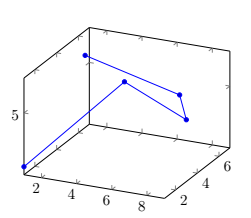
\includegraphics[scale=1.2]{grap}}%
\end{figure}
\end{frame}

\begin{frame}[fragile]{Исходный код}
\begin{adjustbox}{scale=0.8}
\begin{large}
\transwipe

 \begin{lstlisting}[language=Tex]
  \begin{tikzpicture}
\begin{axis}
grid = both,
\addplot3 table [x = b, y = a, z = c] {
	a      b      c
	1      1      1
	7      3      4 
	3      9      5 
	4      8      6
	5      2      7
};
\end{axis}
\end{tikzpicture}

\end{lstlisting}
\end{large}
\end{adjustbox}
\end{frame}



\subsection{Работа с окружениями}
\begin{frame}[label=Back]{Необычное использование таблиц}
\begin{center}
\begin{tabular}{lp{1pt}l} 
    Басалаев Дмитрий && \hspace{2cm} \\\cline{1-1}\cline{3-3} 
     {\tiny Ф.И.О.}     && {\tiny Оценка}
  \end{tabular}
  
  \begin{tabular}{lp{1pt}l} 
    Болковая Полина && \hspace{2cm} \\\cline{1-1}\cline{3-3} 
     {\tiny Ф.И.О.}     && {\tiny Оценка}
  \end{tabular}
  
   \begin{tabular}{lp{1pt}l} 
    Буданцев Артём && \hspace{2cm} \\\cline{1-1}\cline{3-3} 
      {\tiny Ф.И.О.}     && {\tiny Оценка} 
  \end{tabular}
\end{center}
\begin{center}
\hyperlink{Frame}{\beamerbutton{Другой пример}}
\end{center}
\end{frame}




\begin{frame}[fragile]{Исходный код}
\begin{adjustbox}{scale=0.65}
\begin{large}
\transwipe

 \begin{lstlisting}[language=Tex]
  \begin{tabular}{lp{1pt}l} 
    Basalaev Dmitriy && \hspace{2cm} \\cline{1-1}\cline{3-3} 
     {\tiny Full Name}     && {\tiny Grade}
  \end{tabular}

  \begin{tabular}{lp{1pt}l} 
    Bolkovaya Polina && \hspace{2cm} \\cline{1-1}\cline{3-3} 
     {\tiny Full Name}     && {\tiny Grade}
  \end{tabular}

   \begin{tabular}{lp{1pt}l} 
    Budanzev Artem && \hspace{2cm} \\cline{1-1}\cline{3-3} 
      {\tiny Full Name}     && {\tiny Grade} 
  \end{tabular}

\end{lstlisting}
\end{large}
\end{adjustbox}




\end{frame}

\begin{frame}{Использование таблиц при вставке изображений}
\begin{flushleft}


\begin{figure}[h]
\begin{tabular}[scale=0.6]{cc}
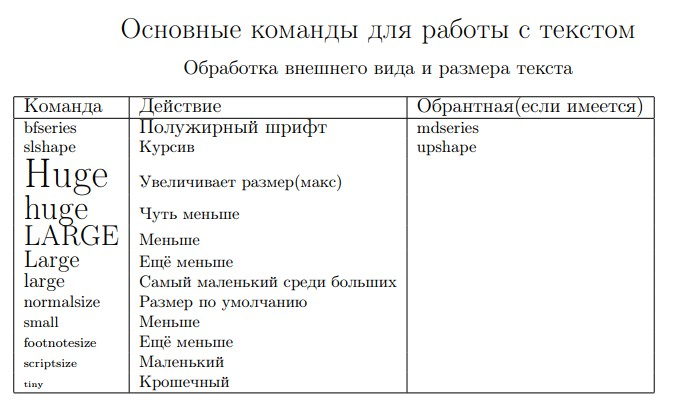
\includegraphics[scale=0.4]{table(1)}
&
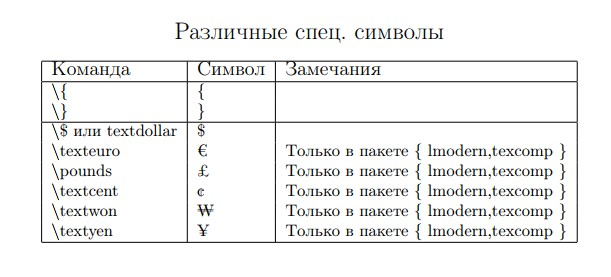
\includegraphics[scale=0.3]{table(2)}
\end{tabular}
\caption{This table}
\end{figure}
\end{flushleft}

\end{frame}
\begin{frame}[fragile]{Исходный код}
\begin{adjustbox}{scale=0.6}
\begin{large}
\transwipe

 \begin{lstlisting}[language=Tex]
  \begin{figure}[h]
\begin{tabular}{cc}
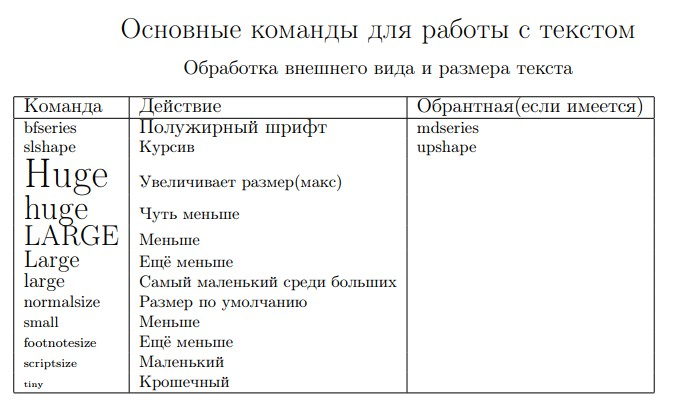
\includegraphics[width=9cm,height=7cm]{table(1)}
&
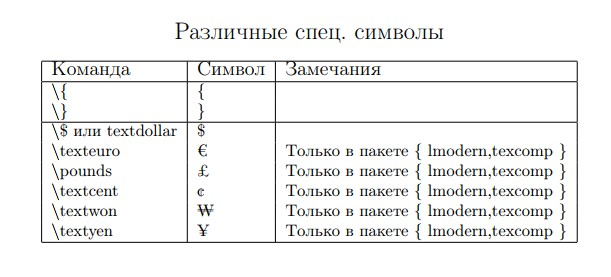
\includegraphics[width=9cm,height=7cm]{table(2)}
\end{tabular}
\caption{This table}
\end{figure}
\newpage
\begin{figure}[h!]
\setlength{\fboxsep}{0pt}
\setlength{\fboxrule}{1pt}
\fbox{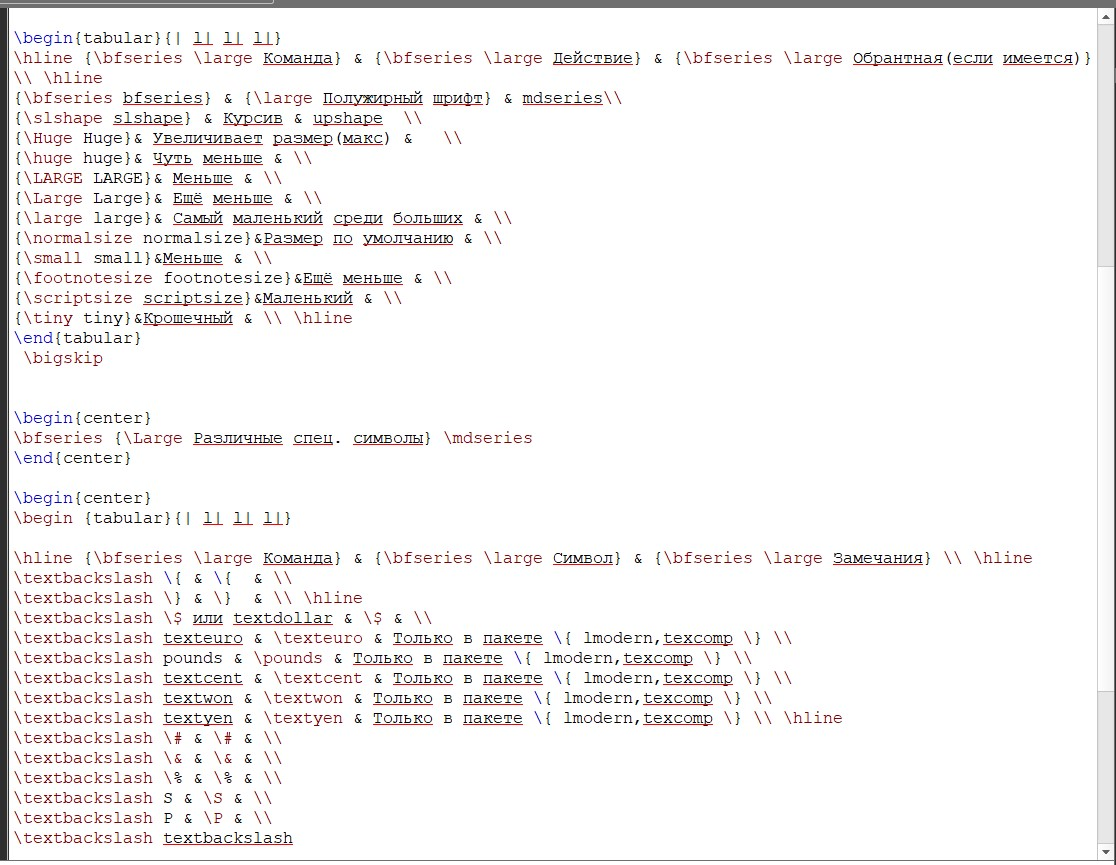
\includegraphics[width=15cm,height=9cm]{TableCode}}
\caption{Table code}
\label{fig:image}
\end{figure}

\end{lstlisting}
\end{large}
\end{adjustbox}
\end{frame}


\begin{frame}{Стандартная таблица}
\begin{tabular}{| l| l| l| l|}
\hline {\bfseries \large N} & {\bfseries \large ФИО} & {\bfseries \large \textsl{группа}} & {\bfseries \large Логин на github.com } \\ \hline
1. & Басалаев Д.А.  & МОА-205 & FySyZe \\ \hline
2. & Болковая П.А.  & МОА-205 & ApollinariaB \\ \hline
3. & Буданцев А.А.  & МОА-205 & Antur1um \\ \hline
\end{tabular}
\end{frame}

\begin{frame}[fragile,label=frame_A]{Исходный код}
\begin{adjustbox}{scale=0.6}
\begin{large}
\transwipe

 \begin{lstlisting}[language=Tex]
  \begin{tabular}{| l| l| l| l|}
\hline {\bfseries \large N} & {\bfseries \large Full Name}
& {\bfseries 
\large \textsl{group}} & 
{\bfseries \large Login on github.com } \\ \hline
1. & Basalaev D.A.  & MOA-205 & FySyZe \\ \hline
2. & Bolkovaya P.A.  & MOA-205 & ApollinariaB \\ \hline
3. & Budantzev A.A.  & MOA-205 & Antur1um \\ \hline
\end{tabular}

\end{lstlisting}
\end{large}
\end{adjustbox}
\end{frame}


\begin{frame}[fragile,label=list]{Исходный код списка}
\begin{adjustbox}{scale=0.7}
\begin{large}
\transwipe

\lstset{extendedchars=\true} %позволяет использовать русские символы в коде

 \begin{lstlisting}[language=Tex]
 \begin{itemize}
  \item[and here you can enter markers
  (by default, these are points)]
   Level 0 Item 0 
  \item Level 0 Item 1 
  \begin{itemize}
    \item Level 1 Item
    \begin{itemize}
      \item Level 2 Item
      \begin{itemize}
        \item Level 3 Item
      \end{itemize}
    \end{itemize}
  \end{itemize}
\end{itemize}
\end{lstlisting}
\end{large}
\end{adjustbox}
\hyperlink{frame_A}{\beamerbutton{Example}}
\end{frame}

\begin{frame}{Verbatin и lstlisting}
\lstinputlisting[language=C++]{Example.cpp}
\end{frame}




\begin{frame}[label=list]{Создание ссылок}

\begin{center}
{\LARGE \textbf{В документе}}
\end{center}

$\textbackslash$ hypertarget \{Уникальный номер ссылки\} 

$\textbackslash$ hyperlink \{Уникальный номер ссылки\} \{ Имя ссылки \}

\begin{center}
{\LARGE \textbf{В презентации}}
\end{center}
$\textbackslash$ begin \{frame\}[label=метка]

$\textbackslash$ hyperlink \{метка нужного слайда\} \\ \{ $\textbackslash$ beamerbutton\{Текст на текст на ``кнопке' \} \}
\end{frame}

\subsection{Работа с презентациями}


\begin{frame}[fragile]{Преамбула в презентации}
\begin{adjustbox}{scale=0.5}
\begin{large}
\transwipe

\lstset{extendedchars=\true} %позволяет использовать русские символы в коде

 \begin{lstlisting}[language=Tex]
 \documentclass{beamer}[aspectratio=169]
	\usepackage[utf8]{inputenc}
	\usepackage[russian]{babel}
    \usepackage{booktabs} 
    \usepackage{beamerthemesplit}
    \setbeamertemplate{footline}[frame number]
    \usepackage{color}
	\usepackage{pdflscape,multicol,blindtext}
	\usepackage{amsmath}
	\usepackage{subcaption}
	\usepackage{listings}
	\usepackage{longtable}
    \usetheme{PaloAlto}
	\usecolortheme{rose}
	\title[Presentation]{Presentation Name}
	\institute{KemSU}
	\author{Dmitriy Basalaev \and Budantzev Artem \and Bolkovaya Polina}
	\date{28.05.2021}
\end{lstlisting}
\end{large}
\end{adjustbox}

\url{https://hartwork.org/beamer-theme-matrix/}

\end{frame}
\usebackgroundtemplate{\includegraphics[width=\paperwidth,height=\paperheight]{White.jpg}}
\begin{frame}{Анимации переходов}
\usebackgroundtemplate{\includegraphics[width=\paperwidth]{123.jpg}}
\begin{itemize}


\item<1-> blindshorizontal — слайд «разрезается» вертикальными полосами;

\item<2-> blindsvertical — слайд «разрезается» горизонтальными полосами;

\item<3-> boxin — старый слайд «стягивается» в точку по центру экрана;

\item<4-> boxout — новый слайд «растягивается» из точки по центру;

\item<5-> dissolve — слайд сменяется мозаикой;

\item<6-> glitter — смесь dissolve с wipe;

\item<7-> splitverticalin «стягивается» сверху и снизу;

\item<8-> splitverticalout «растягивается» сверху и снизу;

\item<9-> wipe — следующий слайд «выезжает» слева.

\end{itemize}


\end{frame}


\usebackgroundtemplate{\includegraphics[width=\paperwidth,height=\paperheight]{White.jpg}}
\begin{frame}{Блоки}
\begin{block}{block}

\end{block}
\begin{alertblock}{alertblock}
\begin{tikzpicture}[scale=0.7]
\draw[red,ultra thick](,1) arc (20:60:2);
\draw[red,ultra thick](0,0) arc (20:60:1.5);
\draw[thick](2,1) arc (0:-120:2);
\end{tikzpicture}
\end{alertblock}
\begin{exampleblock}{exampleblock}
$ (\arcsin \ x)' = \dfrac{1}{\sqrt{1 - x^2}}  $
\end{exampleblock}

\end{frame}

\begin{frame}{Ещё блоки}

  \begin{definition}
Число $\mathbf{ a \in \mathbb{R}}  $  называется пределом числовой последовательности $\mathbf{{x_{n}}}$ если последовательность $ \mathbf{{x_{n}-a}} $ является бесконечно малой, то есть все её элементы, начиная с некоторого, по модулю меньше любого заранее взятого положительного числа.
  \end{definition}

  \begin{theorem}
  
$$\lim_{x \rightarrow x_0}f(x) = A \  \Leftrightarrow \   \forall \ \varepsilon > 0,$$
$$\ \exists \delta \ >0, |\forall x \ 0<|x-x_0|<\delta \ \Rightarrow |f(x) - A|< \varepsilon   $$
  \end{theorem}

   \begin{proof}
     Текст доказательства.
   \end{proof}

\end{frame}








\usebackgroundtemplate{\includegraphics[width=\paperwidth,height=\paperheight]{white(1).png}}
\begin{frame}{Вставка видео}
\includemedia[
	activate=pageopen,
	width=320pt,height=180pt,
	addresource=video.mp4,
	flashvars={%
		source=video.mp4
		&loop=true}
	]{}{VPlayer.swf}

\end{frame}

\begin{frame}[allowframebreaks]{}
	\frametitle{Содержание}
	\tableofcontents
\end{frame}










\usebackgroundtemplate{\includegraphics[width=\paperwidth,height=\paperheight]{white(1).png}}
\section{Конец}
\begin{frame}{Конец}
\centering
\huge
Спасибо за внимание!

\end{frame}

\end{document}



